\section{Results}
\label{sec:results}

\subsection{Required User Interactions for Coprocessing}
   
\begin{figure}
  \centering
  \begin{subfigure}[b]{0.45\textwidth}
    \includegraphics[scale=0.195]{pictures/pieceofcake.eps}
    %\captionof{figure}{Original geometry for our use case}
    \captionof{figure}{}
    \label{fig:piece}
  \end{subfigure}
  ~
  \begin{subfigure}[b]{0.45\textwidth}
    \includegraphics[scale=0.41]{pictures/res.eps}
    %\captionof{figure}{A final coprocessed picture of our simulation. The simulation was run with 128 layers.}
    %\captionof{figure}{A final coprocessed picture of our simulation.}
    \captionof{figure}{}
    \label{fig:res}
  \end{subfigure}
  \caption{(a) original geometry of our use case\\
  \hspace{8em}(b)  a final coprocessed picture of our simulation}
\end{figure}

Before presenting our results we briefly describe how the user interactions were
performed. The following steps were necessary in order to use the developed
coprocessing technology:


1) The user generates a ``light version'' of the mesh. This step has already been
discussed in section~\ref{sec:pip_conf_tools}. Indeed, the user possesses a CAD (Computer Aided
Design) version of the geometry that is parametrized, it is then possible to
obtain meshes at different spatial resolutions. A ``light mesh'' of small size in
memory and representative of the CAD geometry is obtained. Figure~\ref{fig:piece} represents
the ``light version'' of the mesh used in our experiments.


2) We run a short simulation (normally just a few seconds on a local machine) on the ``light mesh''.
This obtains the informations about the result fields we need to create a
visualisation pipeline in ParaView (e.g. temperature, pressure, velocity). We
could then say that we obtain an ``augmented light mesh''.


3) The mesh and the fields obtained at the end of step 2 are read in ParaView
and the user can define her/his visualisation pipeline. At the end of this step
a simple click in the ParaView interface will create a Python file that
programmatically defines the visualisation operations that will be performed
$in$-$situ$.


4) Finally the real simulation is ran using a full resolution size mesh. The
coprocessing part of the simulation reads the python script containing the
definition of the visualisation pipeline. This step is expected to be
time-consuming.
%, in our environment normally perform during several days in a
%supercomputer.

\subsection{Use Cases}

Our simulations have been run on Ivanoe, an EDF corporate supercomputer,
composed of 1382 nodes, each node having 12 cores for a total of 16584 cores. In
these simulations we associate one MPI process by core and we use from 720 cores up
to 3600 cores. We include two use cases that were run on this supercomputer. The
choice of the cases is motivated by two main factors: the size of the mesh and
the complexity of the visualization pipeline. Let us define in more detail why
these two factors:

1) Mesh size. We chose to use two meshes representing the same geometry but at
different resolutions, one made of 51M hexahedral elements and another of 204M
hexahedrals. In our industrial environment at EDF most simulation engineers use
meshes composed by less than 51M of element, then we chose this mesh size to be
representative of the work performed by an average engineer in his work routine.
Furthermore, a 51M elements mesh more than doubles the size used in the results
presented in~\cite{6092322} for the PHASTA adaptor. On the other side, when researcher
oriented simulations are performed at EDF, they currently contain around 200M
elements. We choose then this size as a research oriented or ``heavy mesh'' kind
of simulation.

2) Pipeline complexity. We define two pipelines aimed to be representative of two
different situations: users just performing simple and light visualization
operations (mainly some slices in a volume) and another using very
time-consuming visualization tasks (mainly performing a volume rendering).

\begin{table}
\centering
\begin{tabular}{|p{1.5cm}|p{3.0cm}|p{2.70cm}|p{1.50cm}|}
\hline
\multicolumn{4}{|c|}{\textbf{USE CASES SUM UP}}\\
\hline
NAME & SIZE & PIPELINE & FIGURES \\
\hline
 %& & & \\
$CASE$\_$A$ & 51M hexahedrals, \newline industrial size case & \textbf{heavy}:
\newline volume rendering, \newline celldatatopointdata \newline and glyphs  &
5a 5c 5e\\
\hline
 %& & & \\
$CASE$\_$B$ & 204M hexahedrals, \newline research size case & \textbf{light}:
\newline 9 slices,\newline celldatatopointdata  & 5b 5d 5f   \\
\hline
\end{tabular}
%\vspace{-0.1in}
\caption{Description of our two use cases.}
\label{fig:tab}
%\end{figure}
\vspace{-0.15in}
\end{table}
In the following we name our uses cases:
$CASE$\_$A$, use case using an average mesh size of 51M hexahedrals and a
visualization pipeline including volume rendering which aims to be very time-consuming.
$CASE$\_$B$, our second use case, contains a light visualization pipeline simply
performing some slices but on a large mesh of 204M hexahedrals.

Table~\ref{fig:tab} summarizes the composition of these use cases. In all our use cases we
run a simulation consisting in a fluid with physical properties identical to
water passing through the mesh. Then the output is generated at each step, for a
total of 10 coprocessed visualization images.

%\vspace{-0.10in}
\subsection{Results}

\begin{figure}
        \begin{subfigure}[b]{0.50\textwidth}
                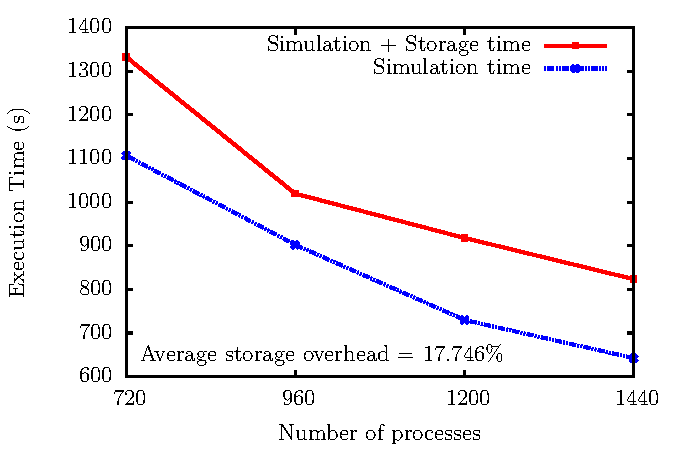
\includegraphics[scale=0.50]{pictures/test41.ps}
                \caption{Time overhead of storage}
                \label{fig:over}
        \end{subfigure}
        ~
        \begin{subfigure}[b]{0.50\textwidth}
                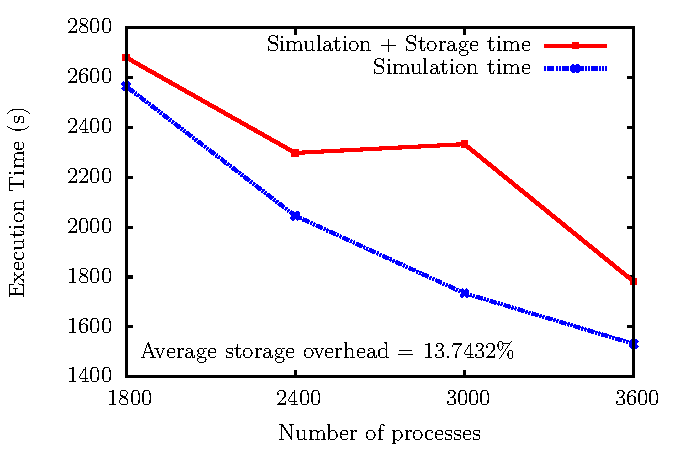
\includegraphics[scale=0.50]{pictures/test42.ps}
                \caption{Time overhead of storage}
                \label{fig:204over}
        \end{subfigure}

        \begin{subfigure}[b]{0.50\textwidth}
          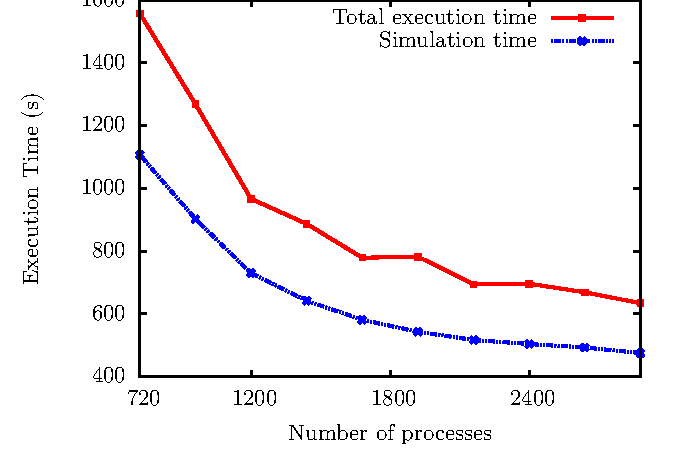
\includegraphics[scale=0.50]{pictures/test1.ps}
                \caption{Execution time with/out coprocessing}
                \label{fig:copro}
        \end{subfigure}%
        ~
        \begin{subfigure}[b]{0.50\textwidth}
          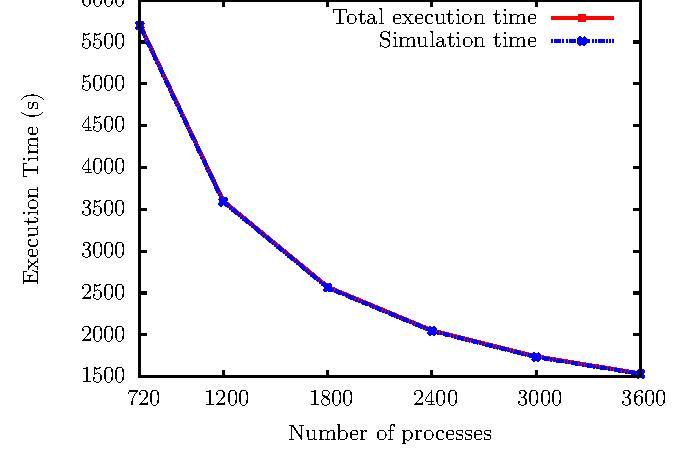
\includegraphics[scale=0.50]{pictures/test12.ps}
                \caption{Execution time with/out coprocessing}
                \label{fig:204copro}
        \end{subfigure}%

        \begin{subfigure}[b]{0.50\textwidth}
                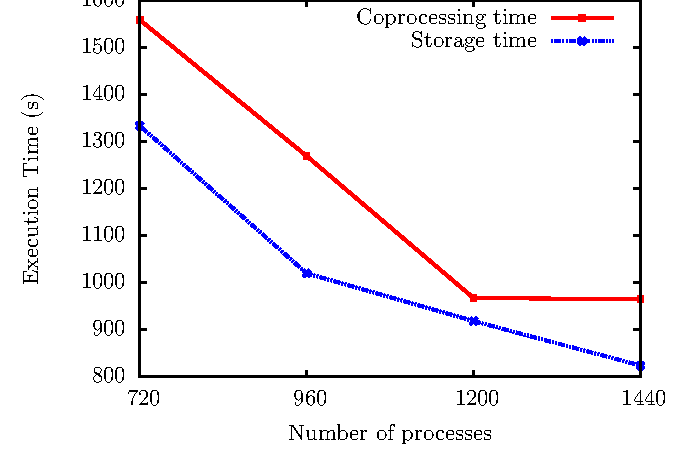
\includegraphics[scale=0.50]{pictures/test2.ps}
                \caption{Execution time comparison with storage.}
                \label{fig:ensight}
        \end{subfigure}
        ~
        \begin{subfigure}[b]{0.50\textwidth}
                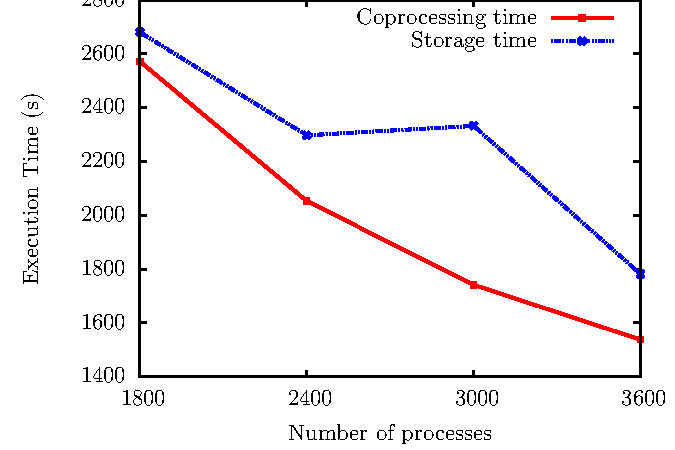
\includegraphics[scale=0.50]{pictures/test22.ps}
                \caption{Execution time comparison with storage.}
                \label{fig:204ensight}
        \end{subfigure}
        \caption{CASE\_A (left) and CASE\_B (right) results}\label{fig:animals}
\end{figure}

Figure~\ref{fig:res} presents an image obtained from one of our $in$-$situ$
simulations with $CASE$\_$A$.
We see the flux of water moving around the vertical cylinders, the glyphs being attached 
to the velocity vectorial field. The color of the volume rendering represents 
the turbulent viscosity of the fluid. 

We establish first the overhead induced by storing our simulation results in
figure~\ref{fig:over} and~\ref{fig:204over}. We observe an average of 18\% and
14\% of time used to store results, for $CASE$\_$A$ and $CASE$\_$B$
respectively. These figures correspond to the comparison of $T_w$ and $T_s + T_w$ in equation 1. 
This overhead tends to increase with the number of processes in
use. It is also not stable and subject to important variations with a peak at
26\%. We thus emphasize the storing process as a bottleneck in every day CFD
studies for its average overhead and its high instability in execution time.

Figure~\ref{fig:copro} shows two graphs of $CASE$\_$A$: in red the execution 
time versus the number of cores, in blue the execution time without
the coprocessing overload. These figures correspond to the comparison of $T_s$ and $T_s + T_{process}$ in equation 2.
We are satisfied by this overload that is contained between 20 and 30\% of the total execution time, 
when we chose complicated task with a high $T_{process}$.
Moreover, it looks like this overload is reducing with the increase in number of cores. 
Figure~\ref{fig:204copro} shows the exact same behavior but with $CASE$\_$B$. Both
graphs are difficult to distinguish as the time needed for coprocessing is
circumscribed between 6 and 10 seconds, the overload (the difference between $T_s$ and $T_s + T_{process}$) is lesser than one
percent of the total execution time. We remark that having heavy $T_{process}$ is not very usual in our applications and 
we include $CASE$\_$A$ as an example of worst case.

We also decided to compare the Catalyst overhead with a non-VTK-based 
storage strategy that performs no visualization operations. Figure~\ref{fig:ensight} and~\ref{fig:204ensight}, 
show the comparison of the global execution time with Catalyst coprocessing
versus the simple Ensight Gold format storage. This means comparing $T_s + T_w$ 
and $T_s + T_{process} + T_{w-in-situ}$. Figure~\ref{fig:ensight} presents
our implementation results with $CASE$\_$A$. This compares positively for Catalyst as the overhead
is approximately 10\% and looks decreasing when the number of cores increase. We
remark that for $CASE$\_$A$ the heavy $T_{process}$ is already taken into
account in the $in-situ$ curve but $T_r + T_v$ is still not performed for the
traditional visualisation scheme. This means that this results is very positive
and we should not forget that $T_r + T_v$ is very time consuming for this case
(and saturates our scientific PCs at EDF R\&D). Figure~\ref{fig:204ensight}
presents our results for $CASE$\_$B$. Here we can see the potential of Catalyst
when 
lighter and more relevant visualization tasks are processed. Indeed, there is no more 
overhead as we gain an average of 10\% of execution time while freeing
ourselves from storage issues (we evaluate the execution time peak of
3000 processes as a result of concurrent accesses on our 
supercomputer storage disks). To emphasize this, Table~\ref{fig:size_tab} shows how much data each
solution generates, namely a basic storage in Ensight Gold format versus our
coprocessing implementation using Catalyst. These informations are those of our
CASE\_B when performing a 10 steps simulation. Both size are
expected to grow proportionally to the size of the mesh input, and the number of
steps. Therefore, we expect the gain provided by the use of coprocessing 
to be increasingly interesting when moving forward in use case size.

%Finally, we also show the total memory use when running $in$-$situ$ visualization
%compared to writing simulation results in Ensight Gold format in
%figure~\ref{fig:over} and~\ref{fig:204over}. We observe that memory consumption
%is increased by an approximate factor varying from 2 to 3. This can be
%explained by both our first naive memory management approach and also by a
%natural increase in memory consumption when visualization operations are to be
%performed. Indeed, our memory management implies a consumption increased by more
%than 2,
%as we need to translate data for Catalyst but still need the former data to
%pursue our simulation. Finally it may also be taken into account the actual memory consumption of the
%chosen visualization tasks. 
%\begin{figure}[!h]
\begin{table}[!h]
\centering
\begin{tabular}{|p{3.5cm}|p{3.5cm}|}
\hline
\multicolumn{2}{|c|}{\textbf{*PROCESSING SIZE COMPARISON}}\\
\hline
STORAGE & COPROCESSING \\
\hline 
 %& \\
57Gio & 1,3Mio \\
\hline 
\end{tabular} 
%\vspace{-0.1in}
\caption{CASE\_B comparison between the size of processed results and simple storage. The simulation was run on 10 steps, with 10
pictures coprocessed.}
\label{fig:size_tab}
%\end{figure}
\end{table}


%\vspace{+0.04in}
%~\

%\clearpage
%\begin{minipage}[t]{\textwidth}
%\begin{minipage}{0.45\linewidth}
%\includegraphics[width=\linewidth]{/home/C26973/res.eps}
%\hspace{0.45in}
%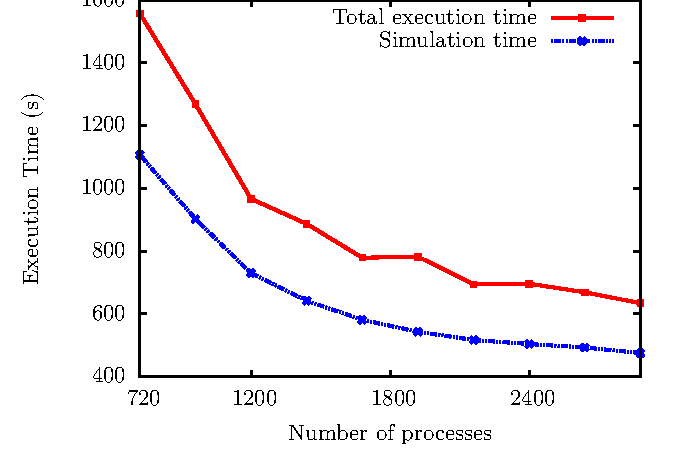
\includegraphics[scale=0.65]{pictures/test1.ps}
%\captionof{figure}{CASE\_A total execution time with and without the coprocessing.}
%\label{fig:copro}
%\vspace{+0.04in}
%~\
%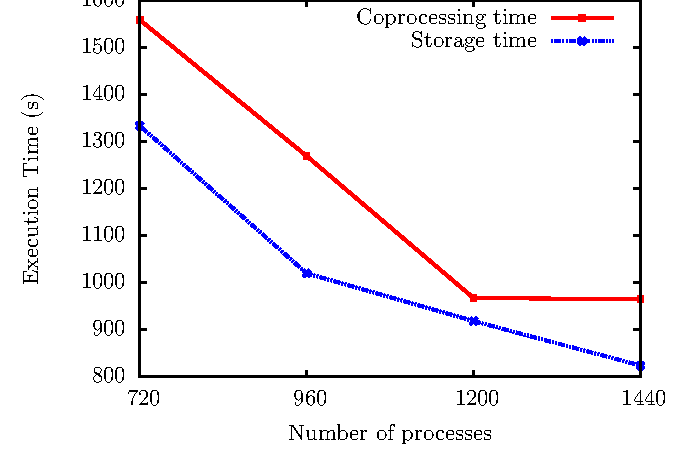
\includegraphics[scale=0.65]{pictures/test2.ps}
%\captionof{figure}{CASE\_A total execution time when using coprocessing and storage in
%Ensight Gold format.}
%\label{fig:ensight}
%\vspace{+0.04in}
%~\
%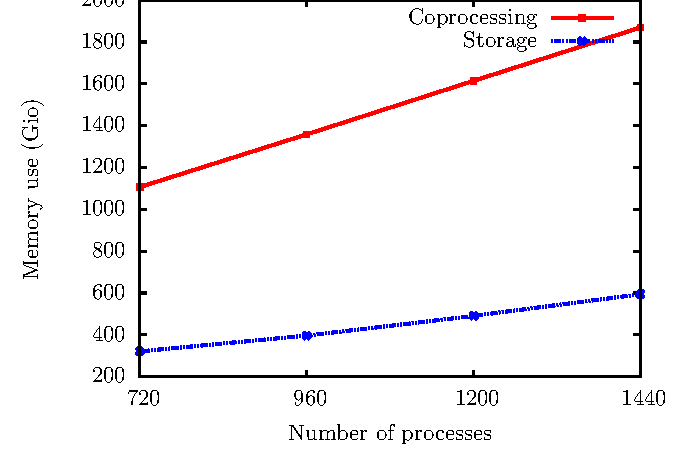
\includegraphics[scale=0.65]{pictures/test3.ps}
%\captionof{figure}{CASE\_A total memory usage when using coprocessing and storage in
%Ensight Gold format.}
%\label{fig:mem}
%\end{minipage}
%\hspace{0.05\linewidth}
%\begin{minipage}{0.45\linewidth}
%\includegraphics[width=\linewidth]{/home/C26973/pieceofcake.eps}
%\hspace{0.65in}
%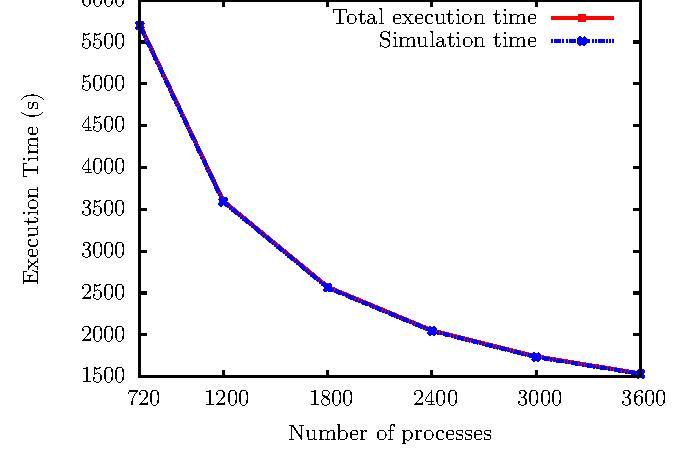
\includegraphics[scale=0.65]{pictures/test12.ps}
%\captionof{figure}{CASE\_B total execution time with and without the coprocessing.}
%\label{fig:204copro}
%\vspace{+0.04in}
%~\
%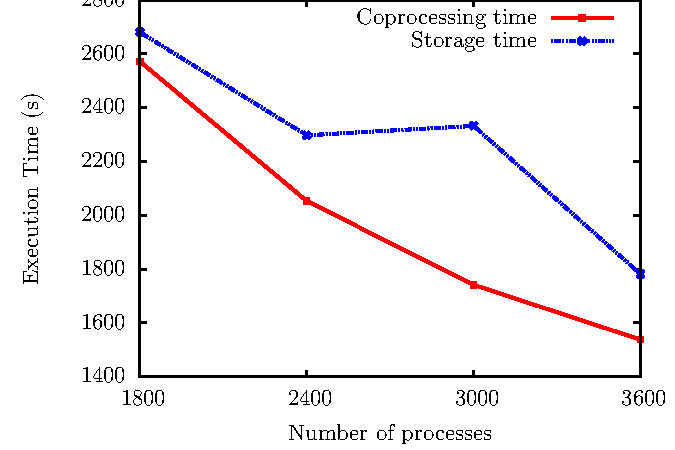
\includegraphics[scale=0.65]{pictures/test22.ps}
%\captionof{figure}{CASE\_B total execution time when using coprocessing and storage in
%Ensight Gold format.}
%\label{fig:204ensight}
%\vspace{+0.04in}
%~\
%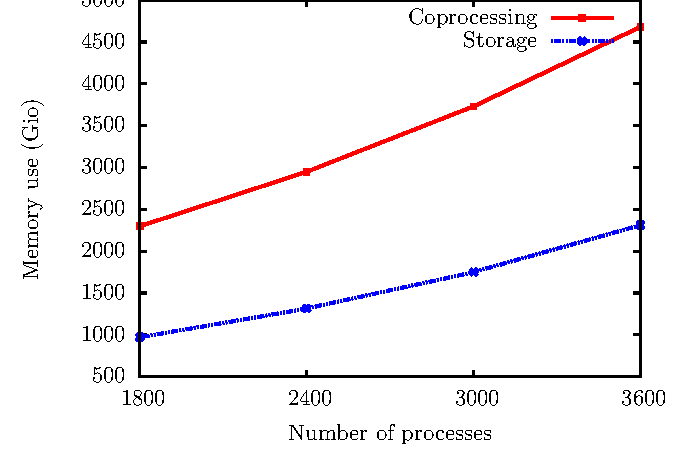
\includegraphics[scale=0.65]{pictures/test32.ps}
%\captionof{figure}{CASE\_B total memory usage when using coprocessing and storage in
%Ensight Gold format.}
%\label{fig:204mem}
%\end{minipage}
%\end{minipage}

        %\caption{CASE\_A results}\label{fig:animals}
%\end{figure}
%~
%\begin{figure}



%\clearpage
